\documentclass[twoside]{book}

% Packages required by doxygen
\usepackage{calc}
\usepackage{doxygen}
\usepackage{graphicx}
\usepackage[utf8]{inputenc}
\usepackage{makeidx}
\usepackage{multicol}
\usepackage{multirow}
\usepackage{textcomp}
\usepackage[table]{xcolor}

% Font selection
\usepackage[T1]{fontenc}
\usepackage{mathptmx}
\usepackage[scaled=.90]{helvet}
\usepackage{courier}
\usepackage{amssymb}
\usepackage{sectsty}
\renewcommand{\familydefault}{\sfdefault}
\allsectionsfont{%
  \fontseries{bc}\selectfont%
  \color{darkgray}%
}
\renewcommand{\DoxyLabelFont}{%
  \fontseries{bc}\selectfont%
  \color{darkgray}%
}

% Page & text layout
\usepackage{geometry}
\geometry{%
  a4paper,%
  top=2.5cm,%
  bottom=2.5cm,%
  left=2.5cm,%
  right=2.5cm%
}
\tolerance=750
\hfuzz=15pt
\hbadness=750
\setlength{\emergencystretch}{15pt}
\setlength{\parindent}{0cm}
\setlength{\parskip}{0.2cm}
\makeatletter
\renewcommand{\paragraph}{%
  \@startsection{paragraph}{4}{0ex}{-1.0ex}{1.0ex}{%
    \normalfont\normalsize\bfseries\SS@parafont%
  }%
}
\renewcommand{\subparagraph}{%
  \@startsection{subparagraph}{5}{0ex}{-1.0ex}{1.0ex}{%
    \normalfont\normalsize\bfseries\SS@subparafont%
  }%
}
\makeatother

% Headers & footers
\usepackage{fancyhdr}
\pagestyle{fancyplain}
\fancyhead[LE]{\fancyplain{}{\bfseries\thepage}}
\fancyhead[CE]{\fancyplain{}{}}
\fancyhead[RE]{\fancyplain{}{\bfseries\leftmark}}
\fancyhead[LO]{\fancyplain{}{\bfseries\rightmark}}
\fancyhead[CO]{\fancyplain{}{}}
\fancyhead[RO]{\fancyplain{}{\bfseries\thepage}}
\fancyfoot[LE]{\fancyplain{}{}}
\fancyfoot[CE]{\fancyplain{}{}}
\fancyfoot[RE]{\fancyplain{}{\bfseries\scriptsize Generated on Wed Dec 23 2015 19\-:13\-:19 for Face\-\_\-detection by Doxygen }}
\fancyfoot[LO]{\fancyplain{}{\bfseries\scriptsize Generated on Wed Dec 23 2015 19\-:13\-:19 for Face\-\_\-detection by Doxygen }}
\fancyfoot[CO]{\fancyplain{}{}}
\fancyfoot[RO]{\fancyplain{}{}}
\renewcommand{\footrulewidth}{0.4pt}
\renewcommand{\chaptermark}[1]{%
  \markboth{#1}{}%
}
\renewcommand{\sectionmark}[1]{%
  \markright{\thesection\ #1}%
}

% Indices & bibliography
\usepackage{natbib}
\usepackage[titles]{tocloft}
\setcounter{tocdepth}{3}
\setcounter{secnumdepth}{5}
\makeindex

% Custom commands
\newcommand{\clearemptydoublepage}{%
  \newpage{\pagestyle{empty}\cleardoublepage}%
}


%===== C O N T E N T S =====

\begin{document}

% Titlepage & ToC
\pagenumbering{roman}
\begin{titlepage}
\vspace*{7cm}
\begin{center}%
{\Large Face\-\_\-detection }\\
\vspace*{1cm}
{\large Generated by Doxygen 1.8.6}\\
\vspace*{0.5cm}
{\small Wed Dec 23 2015 19:13:19}\\
\end{center}
\end{titlepage}
\clearemptydoublepage
\tableofcontents
\clearemptydoublepage
\pagenumbering{arabic}

%--- Begin generated contents ---
\chapter{File Index}
\section{File List}
Here is a list of all files with brief descriptions\-:\begin{DoxyCompactList}
\item\contentsline{section}{src/{\bf face\-\_\-detect.\-cpp} }{\pageref{face__detect_8cpp}}{}
\item\contentsline{section}{src/{\bf image\-\_\-publish.\-cpp} }{\pageref{image__publish_8cpp}}{}
\item\contentsline{section}{src/{\bf imgsubcriber.\-cpp} }{\pageref{imgsubcriber_8cpp}}{}
\item\contentsline{section}{src/{\bf webcam\-\_\-video\-\_\-show.\-cpp} }{\pageref{webcam__video__show_8cpp}}{}
\end{DoxyCompactList}

\chapter{File Documentation}
\section{src/face\-\_\-detect.cpp File Reference}
\label{face__detect_8cpp}\index{src/face\-\_\-detect.\-cpp@{src/face\-\_\-detect.\-cpp}}
{\ttfamily \#include $<$ros/ros.\-h$>$}\\*
{\ttfamily \#include $<$iostream$>$}\\*
{\ttfamily \#include $<$stdio.\-h$>$}\\*
{\ttfamily \#include $<$cv\-\_\-bridge/cv\-\_\-bridge.\-h$>$}\\*
{\ttfamily \#include $<$sensor\-\_\-msgs/image\-\_\-encodings.\-h$>$}\\*
{\ttfamily \#include $<$image\-\_\-transport/image\-\_\-transport.\-h$>$}\\*
{\ttfamily \#include $<$opencv2/objdetect/objdetect.\-hpp$>$}\\*
{\ttfamily \#include $<$opencv2/imgproc/imgproc.\-hpp$>$}\\*
{\ttfamily \#include $<$opencv2/highgui/highgui.\-hpp$>$}\\*
Include dependency graph for face\-\_\-detect.\-cpp\-:
\nopagebreak
\begin{figure}[H]
\begin{center}
\leavevmode
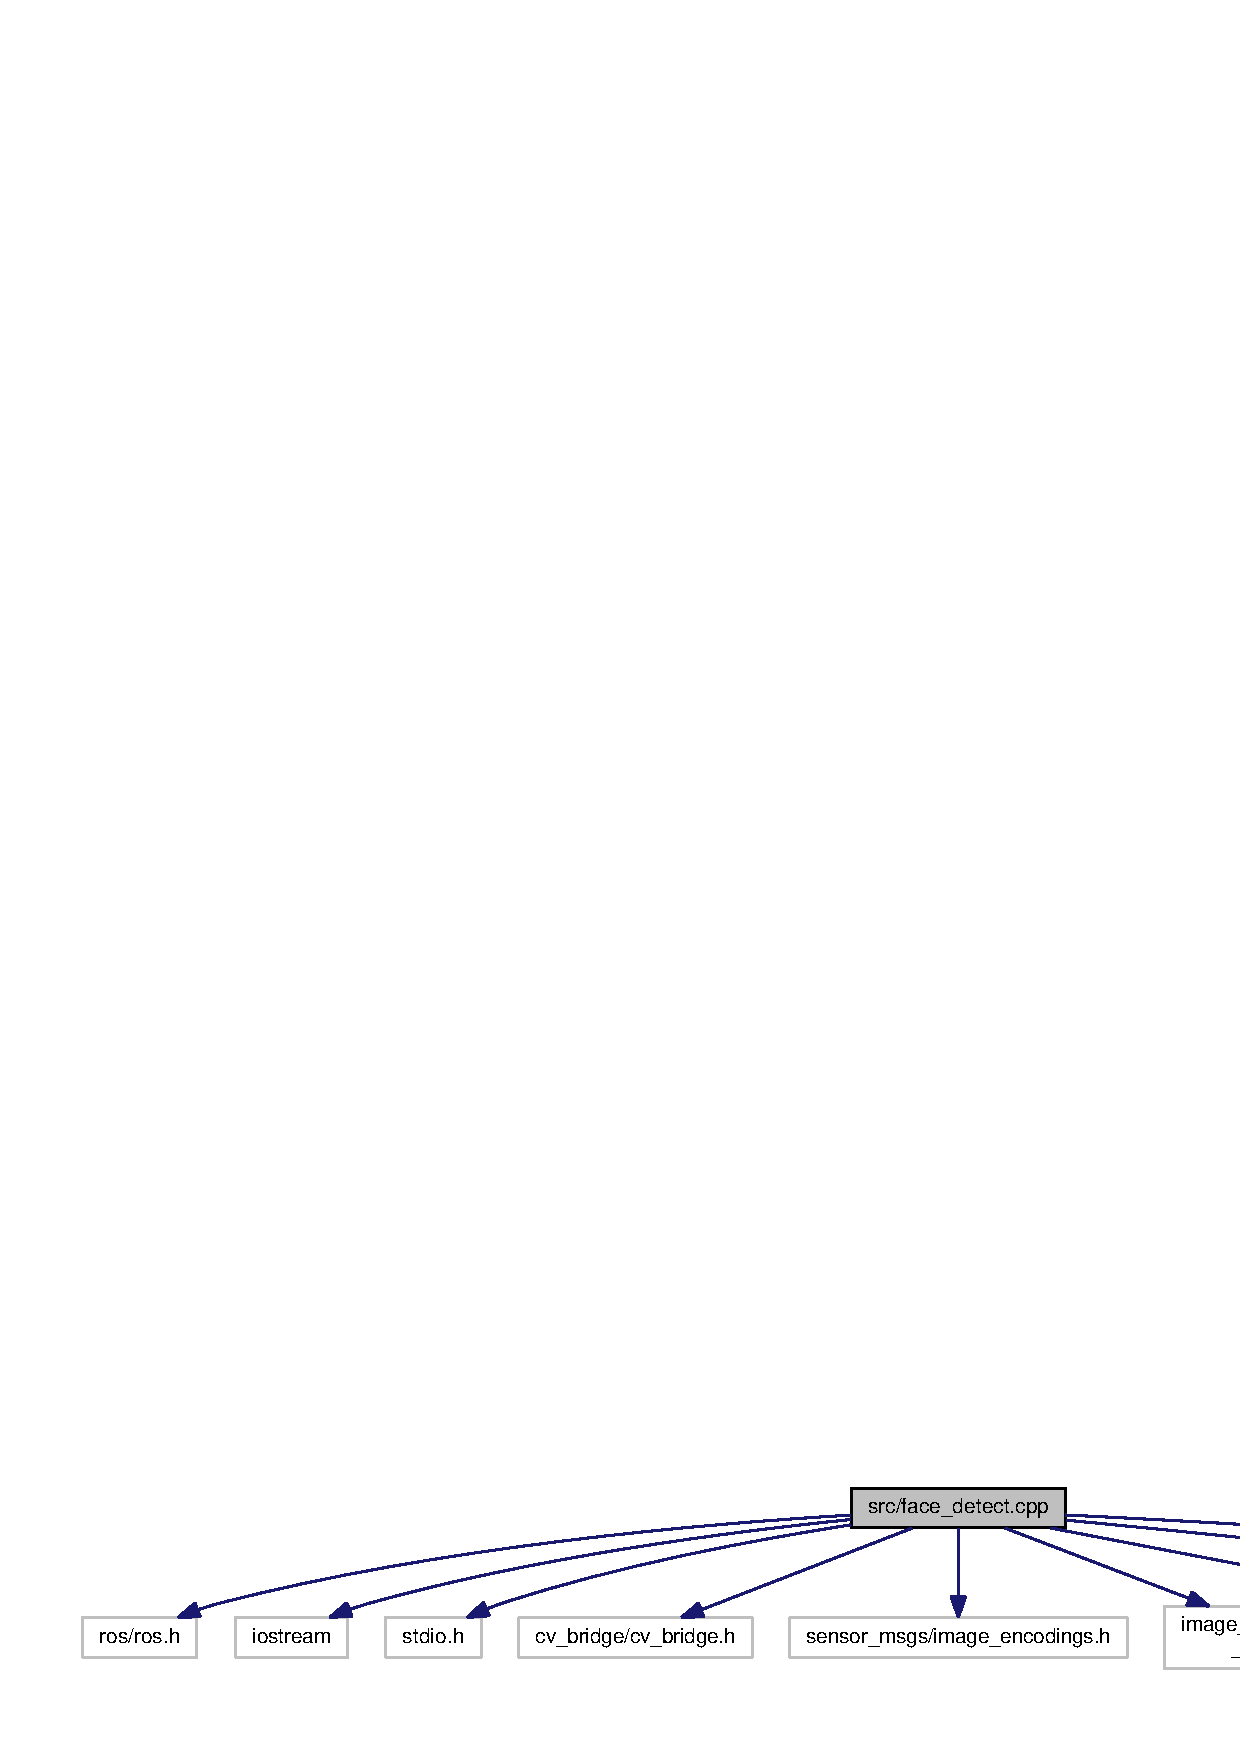
\includegraphics[width=350pt]{face__detect_8cpp__incl}
\end{center}
\end{figure}
\subsection*{Functions}
\begin{DoxyCompactItemize}
\item 
Cascade\-Classifier {\bf face\-\_\-cascade} (\char`\"{}/home/gokul/catkin\-\_\-ws/src/face\-\_\-detection/share/facetracking/haarcascade\-\_\-frontalface\-\_\-default.\-xml\char`\"{})
\item 
void {\bf image\-Callback} (const sensor\-\_\-msgs\-::\-Image\-Const\-Ptr \&original\-\_\-image)
\item 
int {\bf main} (int argc, char $\ast$$\ast$argv)
\end{DoxyCompactItemize}
\subsection*{Variables}
\begin{DoxyCompactItemize}
\item 
image\-\_\-transport\-::\-Publisher {\bf pub}
\end{DoxyCompactItemize}


\subsection{Function Documentation}
\index{face\-\_\-detect.\-cpp@{face\-\_\-detect.\-cpp}!face\-\_\-cascade@{face\-\_\-cascade}}
\index{face\-\_\-cascade@{face\-\_\-cascade}!face_detect.cpp@{face\-\_\-detect.\-cpp}}
\subsubsection[{face\-\_\-cascade}]{\setlength{\rightskip}{0pt plus 5cm}Cascade\-Classifier face\-\_\-cascade (
\begin{DoxyParamCaption}
\item[{\char`\"{}/home/gokul/catkin\-\_\-ws/src/face\-\_\-detection/share/facetracking/haarcascade\-\_\-frontalface\-\_\-default.\-xml\char`\"{}}]{}
\end{DoxyParamCaption}
)}\label{face__detect_8cpp_ac44a6f7253ef9bf766726a7f4e4d1076}
\index{face\-\_\-detect.\-cpp@{face\-\_\-detect.\-cpp}!image\-Callback@{image\-Callback}}
\index{image\-Callback@{image\-Callback}!face_detect.cpp@{face\-\_\-detect.\-cpp}}
\subsubsection[{image\-Callback}]{\setlength{\rightskip}{0pt plus 5cm}void image\-Callback (
\begin{DoxyParamCaption}
\item[{const sensor\-\_\-msgs\-::\-Image\-Const\-Ptr \&}]{original\-\_\-image}
\end{DoxyParamCaption}
)}\label{face__detect_8cpp_aee834d16d4f2f1d2b3aacf53333b2309}


Definition at line 30 of file face\-\_\-detect.\-cpp.

\index{face\-\_\-detect.\-cpp@{face\-\_\-detect.\-cpp}!main@{main}}
\index{main@{main}!face_detect.cpp@{face\-\_\-detect.\-cpp}}
\subsubsection[{main}]{\setlength{\rightskip}{0pt plus 5cm}int main (
\begin{DoxyParamCaption}
\item[{int}]{argc, }
\item[{char $\ast$$\ast$}]{argv}
\end{DoxyParamCaption}
)}\label{face__detect_8cpp_a3c04138a5bfe5d72780bb7e82a18e627}


Definition at line 90 of file face\-\_\-detect.\-cpp.



\subsection{Variable Documentation}
\index{face\-\_\-detect.\-cpp@{face\-\_\-detect.\-cpp}!pub@{pub}}
\index{pub@{pub}!face_detect.cpp@{face\-\_\-detect.\-cpp}}
\subsubsection[{pub}]{\setlength{\rightskip}{0pt plus 5cm}image\-\_\-transport\-::\-Publisher pub}\label{face__detect_8cpp_aa3018a2730fde05a0032471af5d5dff2}


Definition at line 25 of file face\-\_\-detect.\-cpp.


\section{src/image\-\_\-publish.cpp File Reference}
\label{image__publish_8cpp}\index{src/image\-\_\-publish.\-cpp@{src/image\-\_\-publish.\-cpp}}
{\ttfamily \#include $<$ros/ros.\-h$>$}\\*
{\ttfamily \#include $<$image\-\_\-transport/image\-\_\-transport.\-h$>$}\\*
{\ttfamily \#include $<$opencv2/highgui/highgui.\-hpp$>$}\\*
{\ttfamily \#include $<$opencv2/imgproc/imgproc.\-hpp$>$}\\*
{\ttfamily \#include $<$cv\-\_\-bridge/cv\-\_\-bridge.\-h$>$}\\*
Include dependency graph for image\-\_\-publish.\-cpp\-:
\nopagebreak
\begin{figure}[H]
\begin{center}
\leavevmode
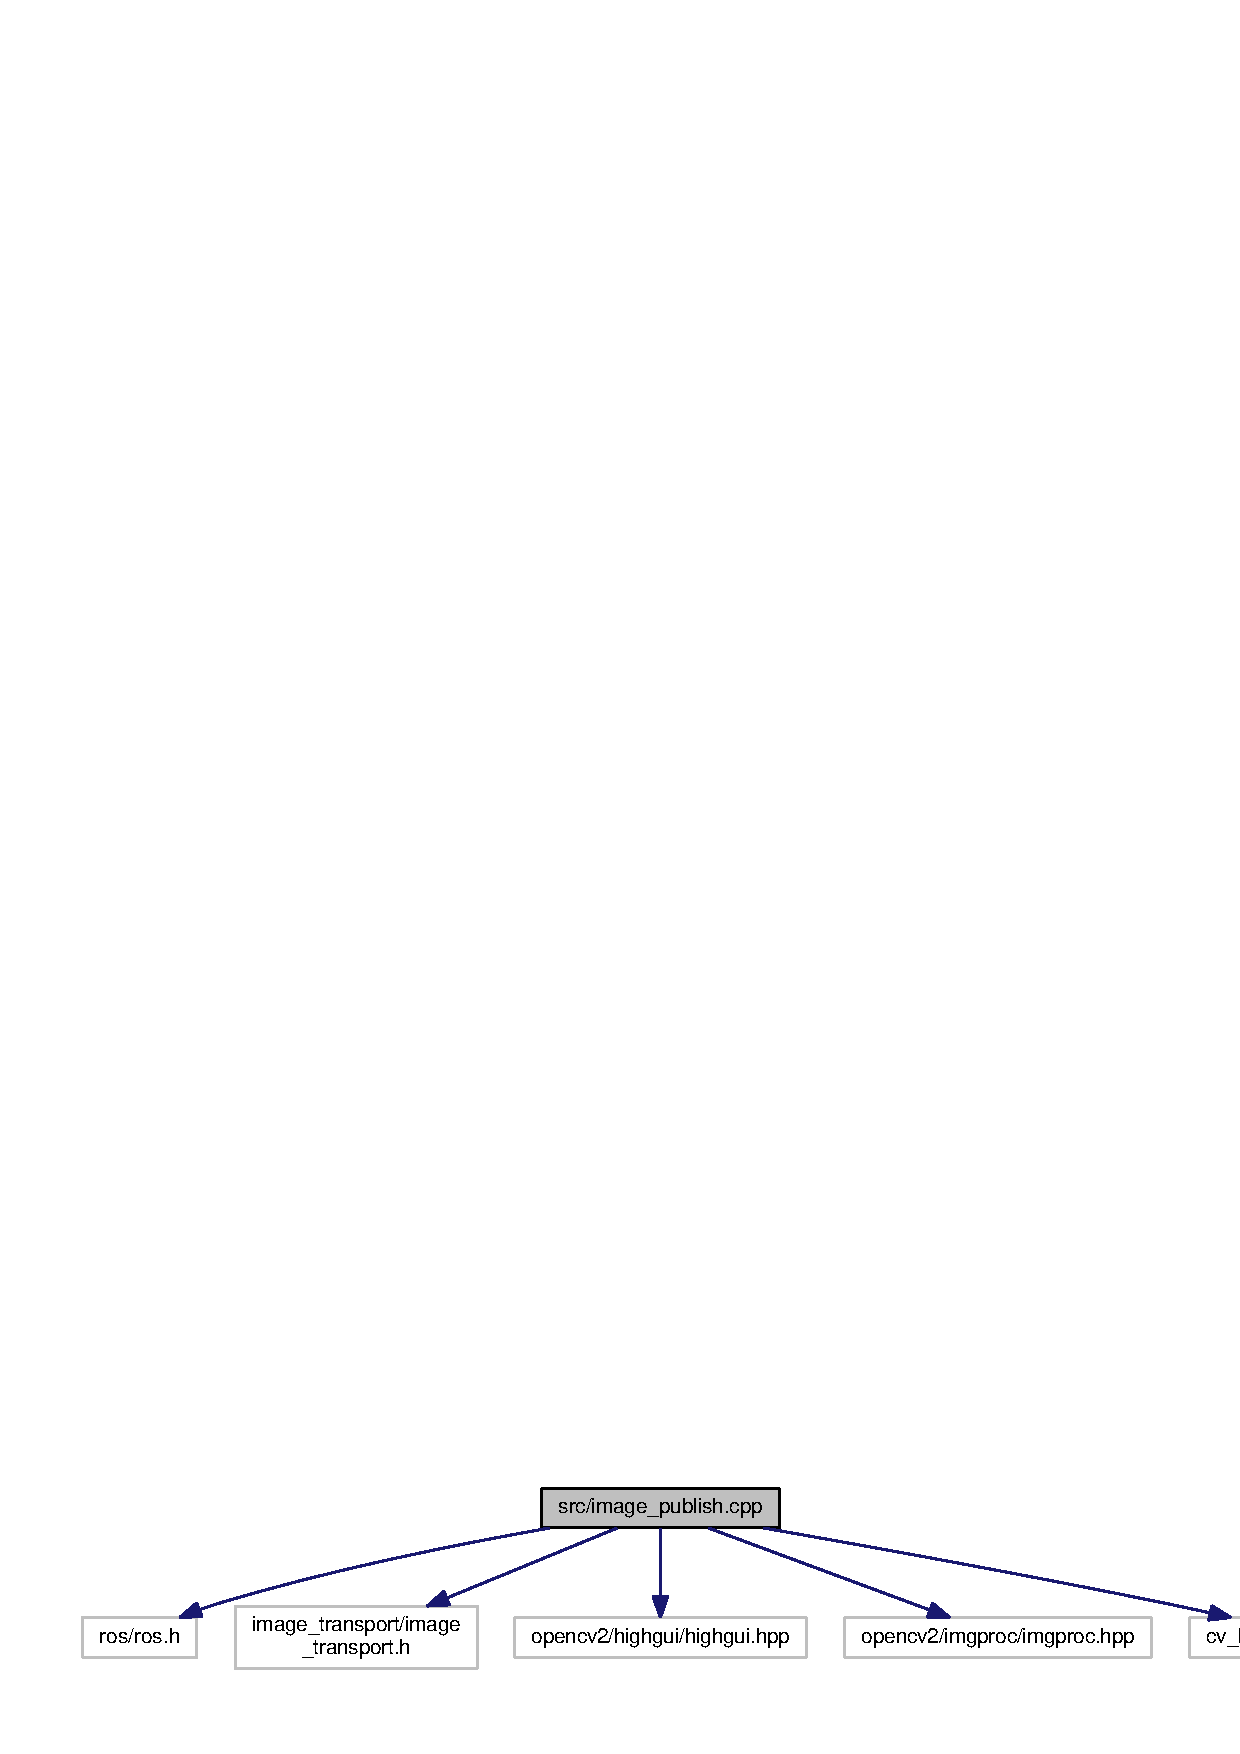
\includegraphics[width=350pt]{image__publish_8cpp__incl}
\end{center}
\end{figure}
\subsection*{Functions}
\begin{DoxyCompactItemize}
\item 
int {\bf main} (int argc, char $\ast$$\ast$argv)
\end{DoxyCompactItemize}
\subsection*{Variables}
\begin{DoxyCompactItemize}
\item 
const float {\bf k\-Scale\-Factor} = 1.\-0
\end{DoxyCompactItemize}


\subsection{Function Documentation}
\index{image\-\_\-publish.\-cpp@{image\-\_\-publish.\-cpp}!main@{main}}
\index{main@{main}!image_publish.cpp@{image\-\_\-publish.\-cpp}}
\subsubsection[{main}]{\setlength{\rightskip}{0pt plus 5cm}int main (
\begin{DoxyParamCaption}
\item[{int}]{argc, }
\item[{char $\ast$$\ast$}]{argv}
\end{DoxyParamCaption}
)}\label{image__publish_8cpp_a3c04138a5bfe5d72780bb7e82a18e627}


Definition at line 17 of file image\-\_\-publish.\-cpp.



\subsection{Variable Documentation}
\index{image\-\_\-publish.\-cpp@{image\-\_\-publish.\-cpp}!k\-Scale\-Factor@{k\-Scale\-Factor}}
\index{k\-Scale\-Factor@{k\-Scale\-Factor}!image_publish.cpp@{image\-\_\-publish.\-cpp}}
\subsubsection[{k\-Scale\-Factor}]{\setlength{\rightskip}{0pt plus 5cm}const float k\-Scale\-Factor = 1.\-0}\label{image__publish_8cpp_a104ca8735e102aef1fa710454137dbc8}


Definition at line 15 of file image\-\_\-publish.\-cpp.


\section{src/imgsubcriber.cpp File Reference}
\label{imgsubcriber_8cpp}\index{src/imgsubcriber.\-cpp@{src/imgsubcriber.\-cpp}}
{\ttfamily \#include $<$ros/ros.\-h$>$}\\*
{\ttfamily \#include $<$image\-\_\-transport/image\-\_\-transport.\-h$>$}\\*
{\ttfamily \#include $<$opencv2/highgui/highgui.\-hpp$>$}\\*
{\ttfamily \#include $<$cv\-\_\-bridge/cv\-\_\-bridge.\-h$>$}\\*
Include dependency graph for imgsubcriber.\-cpp\-:
\nopagebreak
\begin{figure}[H]
\begin{center}
\leavevmode
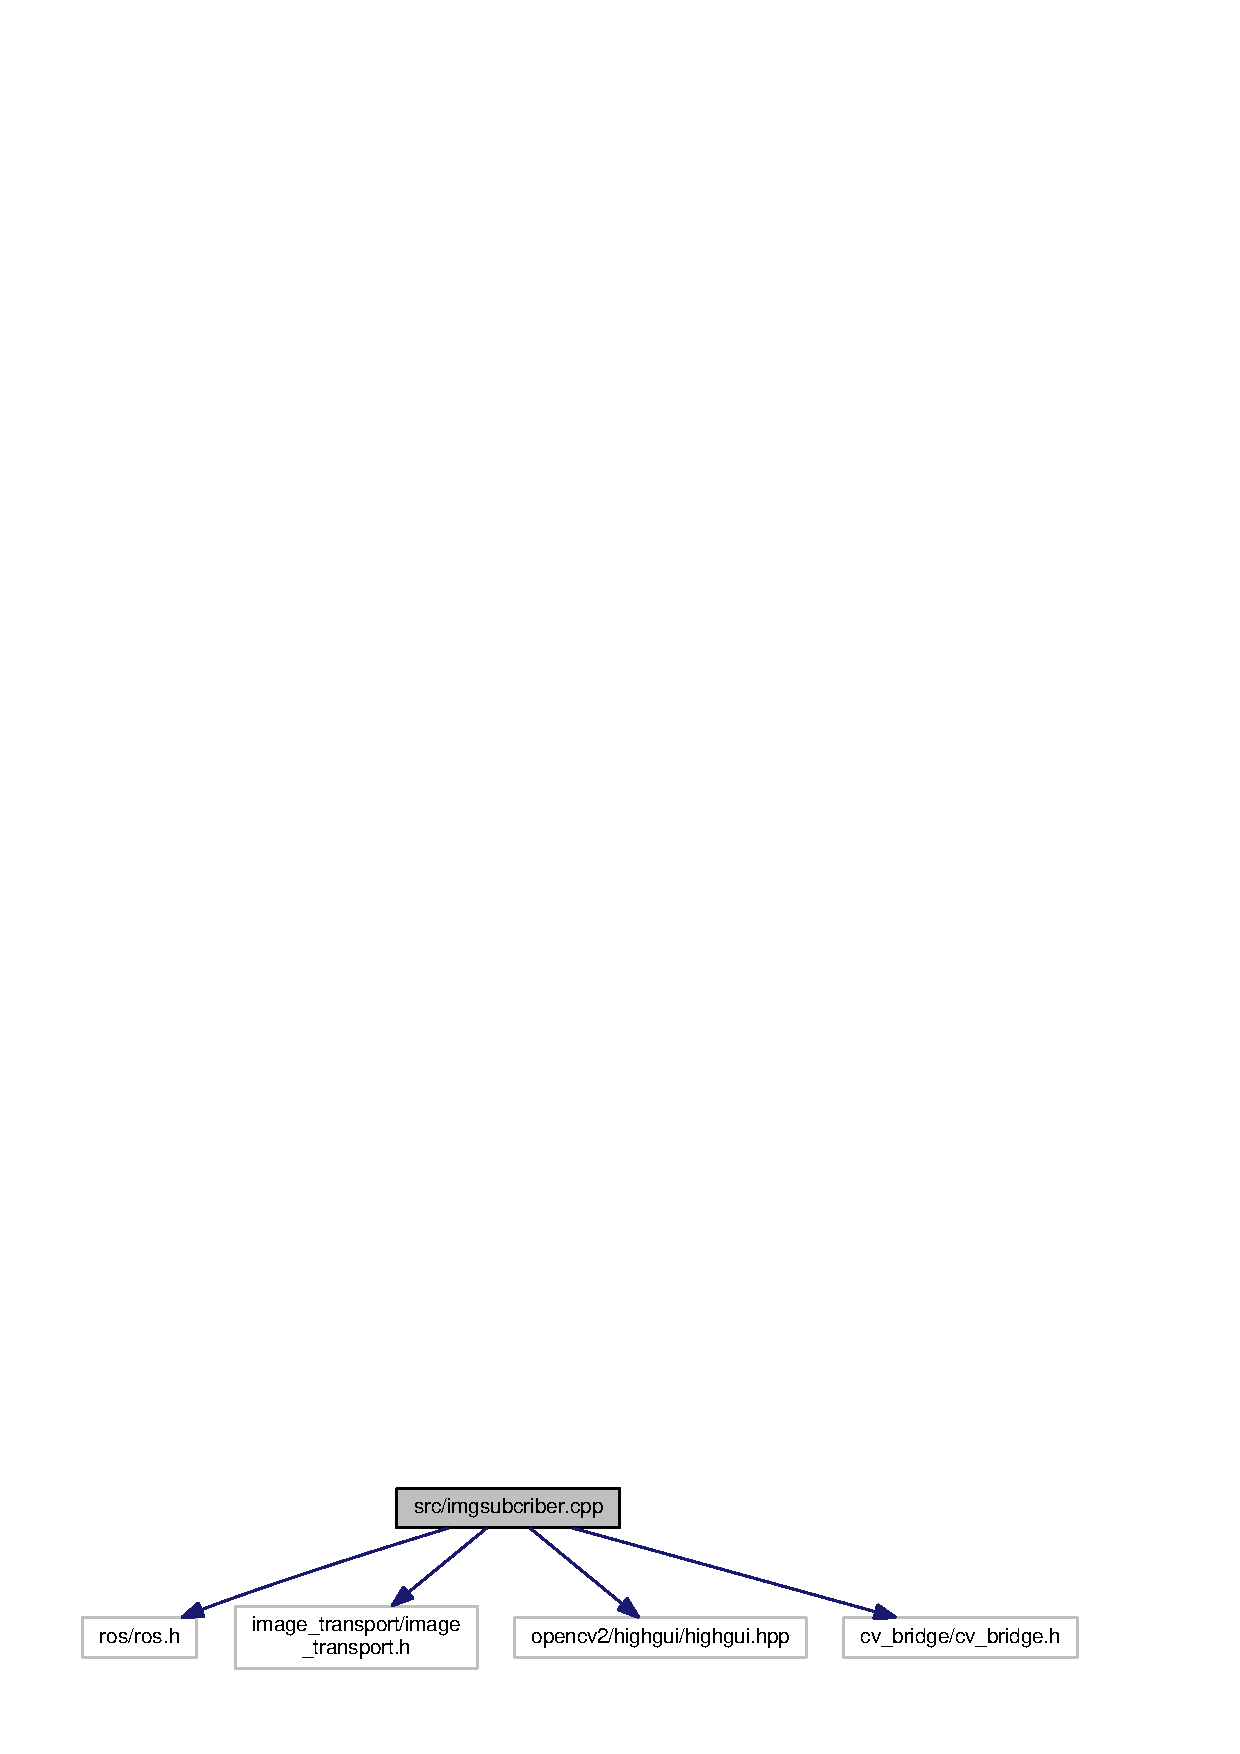
\includegraphics[width=350pt]{imgsubcriber_8cpp__incl}
\end{center}
\end{figure}
\subsection*{Functions}
\begin{DoxyCompactItemize}
\item 
void {\bf image\-Callback} (const sensor\-\_\-msgs\-::\-Image\-Const\-Ptr \&msg)
\item 
int {\bf main} (int argc, char $\ast$$\ast$argv)
\end{DoxyCompactItemize}


\subsection{Function Documentation}
\index{imgsubcriber.\-cpp@{imgsubcriber.\-cpp}!image\-Callback@{image\-Callback}}
\index{image\-Callback@{image\-Callback}!imgsubcriber.cpp@{imgsubcriber.\-cpp}}
\subsubsection[{image\-Callback}]{\setlength{\rightskip}{0pt plus 5cm}void image\-Callback (
\begin{DoxyParamCaption}
\item[{const sensor\-\_\-msgs\-::\-Image\-Const\-Ptr \&}]{msg}
\end{DoxyParamCaption}
)}\label{imgsubcriber_8cpp_a0d7dfd9133ce1e6b48bfdc8249db33d1}


Definition at line 15 of file imgsubcriber.\-cpp.

\index{imgsubcriber.\-cpp@{imgsubcriber.\-cpp}!main@{main}}
\index{main@{main}!imgsubcriber.cpp@{imgsubcriber.\-cpp}}
\subsubsection[{main}]{\setlength{\rightskip}{0pt plus 5cm}int main (
\begin{DoxyParamCaption}
\item[{int}]{argc, }
\item[{char $\ast$$\ast$}]{argv}
\end{DoxyParamCaption}
)}\label{imgsubcriber_8cpp_a3c04138a5bfe5d72780bb7e82a18e627}


Definition at line 32 of file imgsubcriber.\-cpp.


\section{src/webcam\-\_\-video\-\_\-show.cpp File Reference}
\label{webcam__video__show_8cpp}\index{src/webcam\-\_\-video\-\_\-show.\-cpp@{src/webcam\-\_\-video\-\_\-show.\-cpp}}
{\ttfamily \#include $<$ros/ros.\-h$>$}\\*
{\ttfamily \#include $<$image\-\_\-transport/image\-\_\-transport.\-h$>$}\\*
{\ttfamily \#include $<$opencv2/highgui/highgui.\-hpp$>$}\\*
{\ttfamily \#include $<$cv\-\_\-bridge/cv\-\_\-bridge.\-h$>$}\\*
{\ttfamily \#include $<$sstream$>$}\\*
Include dependency graph for webcam\-\_\-video\-\_\-show.\-cpp\-:
\nopagebreak
\begin{figure}[H]
\begin{center}
\leavevmode
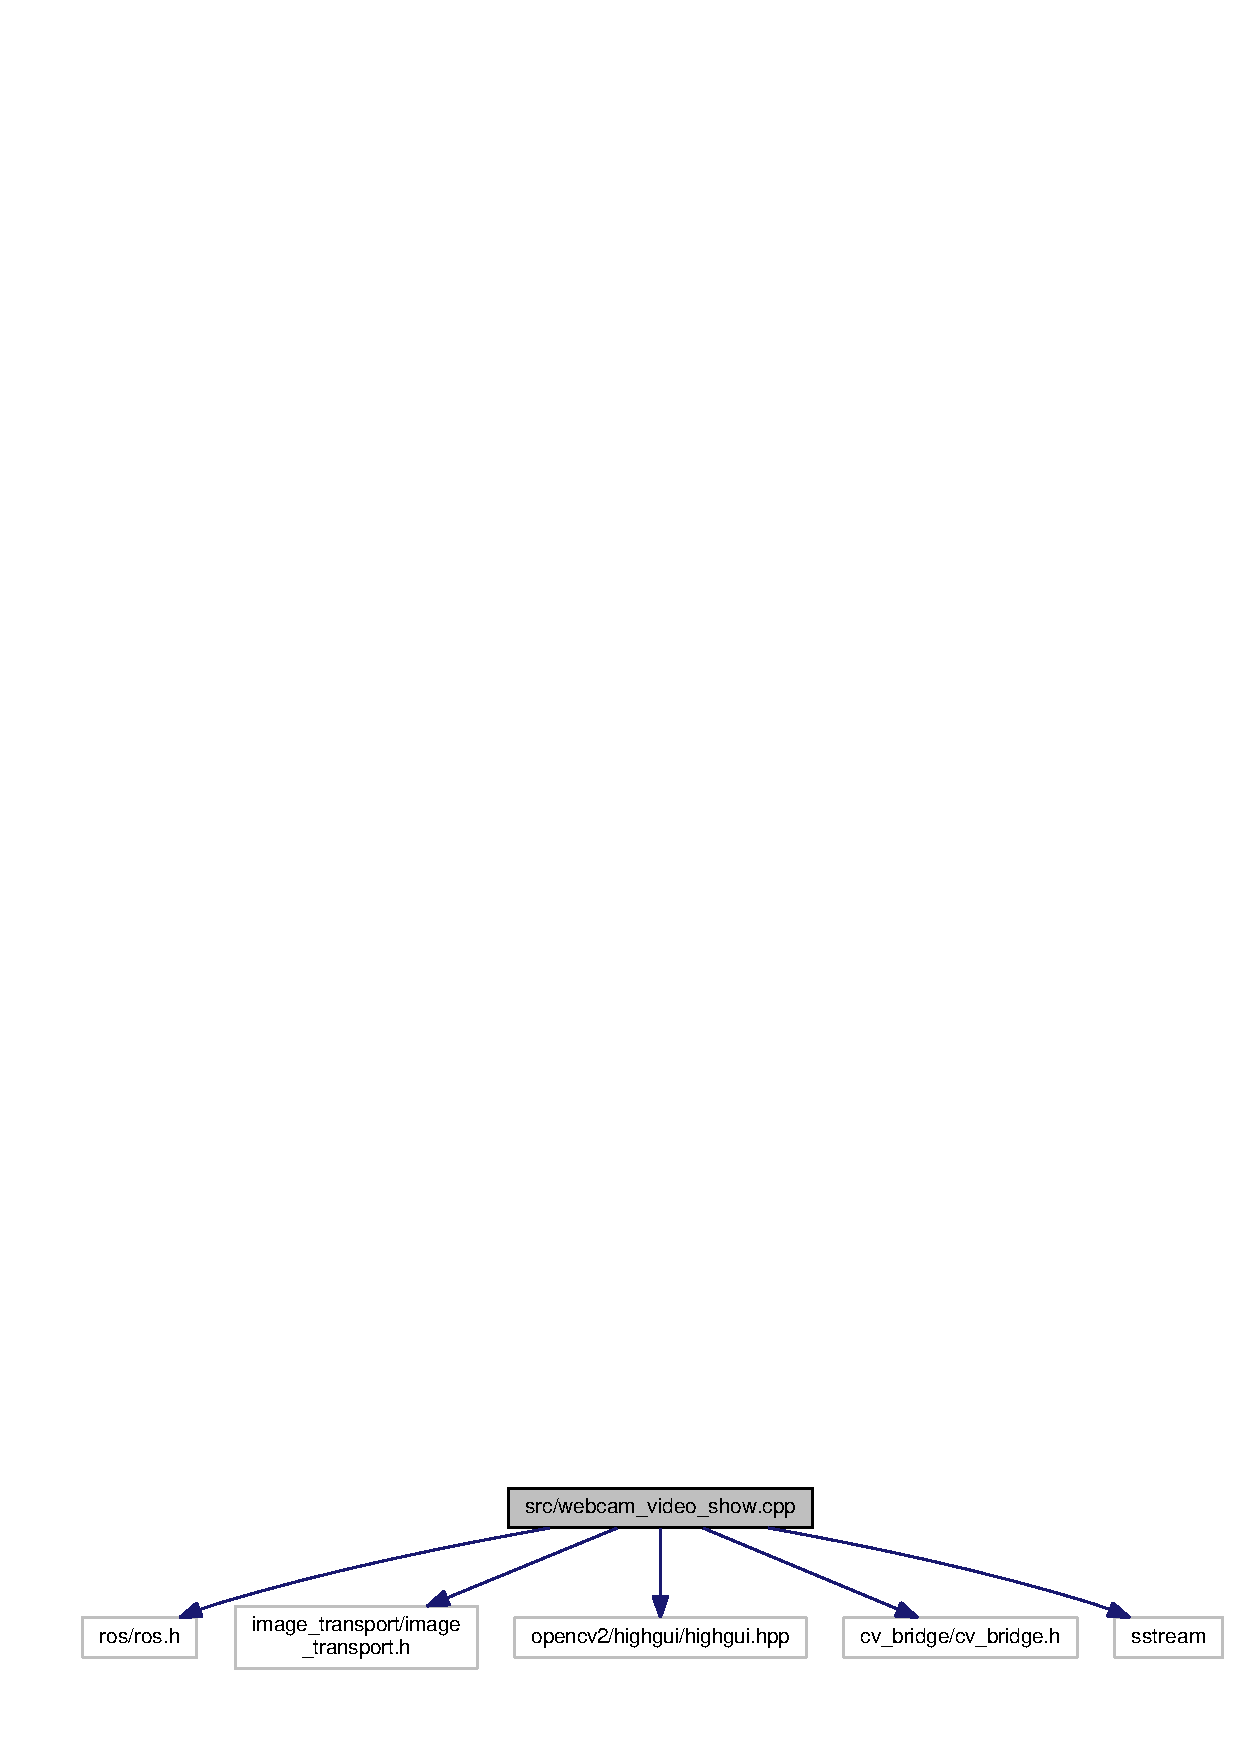
\includegraphics[width=350pt]{webcam__video__show_8cpp__incl}
\end{center}
\end{figure}
\subsection*{Functions}
\begin{DoxyCompactItemize}
\item 
int {\bf main} (int argc, char $\ast$$\ast$argv)
\end{DoxyCompactItemize}


\subsection{Function Documentation}
\index{webcam\-\_\-video\-\_\-show.\-cpp@{webcam\-\_\-video\-\_\-show.\-cpp}!main@{main}}
\index{main@{main}!webcam_video_show.cpp@{webcam\-\_\-video\-\_\-show.\-cpp}}
\subsubsection[{main}]{\setlength{\rightskip}{0pt plus 5cm}int main (
\begin{DoxyParamCaption}
\item[{int}]{argc, }
\item[{char $\ast$$\ast$}]{argv}
\end{DoxyParamCaption}
)}\label{webcam__video__show_8cpp_a3c04138a5bfe5d72780bb7e82a18e627}


Definition at line 12 of file webcam\-\_\-video\-\_\-show.\-cpp.


%--- End generated contents ---

% Index
\newpage
\phantomsection
\addcontentsline{toc}{chapter}{Index}
\printindex

\end{document}
